\documentclass[10pt]{beamer}

% ---- Packages ----

\usepackage[utf8]{inputenc}
\usepackage[T1]{fontenc}
\usepackage[spanish]{babel}
\usepackage{epsfig}
\usepackage{graphics}
\usepackage{tabularx}
\usepackage{listings}
\usepackage{float}
\usepackage{multirow}
\usepackage{noto}
\usepackage{eurosym}
\usepackage{epsfig}
\usepackage{amssymb}
\usepackage{amsmath}
\usepackage{xcolor}

% ---- Configuration ----

\usetheme{Madrid}
\useinnertheme{circles}
\usenavigationsymbolstemplate{}
\setbeamertemplate{blocks}[rounded]

\definecolor{UDCpink}{RGB}{214,30,140}
\definecolor{UDCgray}{RGB}{100,100,100}

\usecolortheme[named=UDCpink]{structure}

\makeatletter
\setbeamertemplate{title page}
{
	\vbox{}
	\vspace{0.25em}
	\begin{centering}
		{\usebeamercolor[fg]{titlegraphic}\inserttitlegraphic\par}
		\vspace{1em}
		\begin{beamercolorbox}[sep=8pt,center,rounded=true]{title}
			\usebeamerfont{title}\inserttitle\par%
			\ifx\insertsubtitle\@empty%
			\else%
			\vspace{0.25em}
			{\usebeamerfont{subtitle}\usebeamercolor[fg]{subtitle}\insertsubtitle\par}%
			\fi%     
		\end{beamercolorbox}%
		\vfill
		\begin{beamercolorbox}[sep=8pt,center]{author}
			\usebeamerfont{author}\insertauthor
		\end{beamercolorbox}
		\begin{beamercolorbox}[sep=8pt,center]{institute}
			\usebeamerfont{institute}\insertinstitute
		\end{beamercolorbox}
		\begin{beamercolorbox}[sep=8pt,right]{date}
			\itshape\usebeamerfont{date}\insertdate
		\end{beamercolorbox}
	\end{centering}
	\vspace{0.25em}
}
\makeatother

\lstdefinestyle{myLuastyle}
{
	language         = {[5.2]Lua},
	commentstyle=\color{green},
	keywordstyle=\color{blue}, 
	basicstyle = \ttfamily \color{black} \footnotesize
}

\lstset{style=myLuastyle}

% ---- Document ----

\title[Generación mediante ASP]{Generación de Escenarios de un Videojuego 2D mediante Programación Lógica}
\author[Rafael Alcalde Azpiazu]{\large Rafael Alcalde Azpiazu}
\institute[UDC] % (optional)
{
	\normalsize
	Grado en Ingeniería Informática \\
	Mención en Computación \\
	\vspace{1em}
	Proyecto clásico de Ingeniería \\
	Facultad de Informática \\
	\vspace{1em}
	Director: Pedro Cabalar \\
}
\date[]{A Coruña, \today}
\titlegraphic{
\includegraphics[height=2em]{images/logo.png}}

\begin{document}
	
	\begin{frame}
		\titlepage
	\end{frame}

	\section{Motivación}
	\begin{frame}
	\frametitle{Motivación}

	\begin{itemize}
		\item<1-> La \textcolor{UDCpink}{industria del videojuego} constituye un sector económico cada vez más relevante.
		
		\vspace{0.5em}
		
		\pause
		
		Beneficios netos (en dólares):
		
		\begin{itemize}
			\item Minecraft: 2500 millones, Fornite: 1000 millones, Destiny: 500 millones.
		\end{itemize}
	
		\vspace{1em}
		
		\item<3-> Ha activado avances tecnológicos, p. ej. el uso de la \textcolor{UDCpink}{Inteligencia Artificial}, uno de los campos que más ha contribuido.
		
		\vspace{0.5em}
		
		\begin{itemize}
			\item<4-> Diseño de \textcolor{UDCpink}{enemigos inteligentes}, p. ej mediante programación evolutiva (No Man's Sky).
			
			\vspace{0.5em}
			
			\item<5-> \textcolor{UDCpink}{Diseño del entorno}. Existen dos aproximaciones:
			
			\vspace{0.5em}
			
			\begin{itemize}
				\item<5->\small Generación procedimental. La más usada.
				
				\vspace{0.5em}
				
				\item<6->\small \textcolor{UDCpink}{Generación declarativa} $\Leftarrow$.
			\end{itemize}
		\end{itemize}
	\end{itemize}
\end{frame}

\begin{frame}
	\frametitle{Diseño de entornos}
	
	\begin{itemize}
		\item \textcolor{UDCpink}{Generación procedimental}: se basa en un algoritmo o técnica ya predefinida.
		
		\vspace{1em}
		
		\begin{enumerate}
			\item Algoritmo ad-hoc.
			
			\vspace{0.5em}
			
			\item Programación evolutiva.
			
			\vspace{0.5em}
			
			\item Expresiones matemáticas.
		\end{enumerate}
	\end{itemize}
	
	\vspace{1em}
	
	\pause
	
	\begin{block}{\normalsize Problemática}
		\vspace{1em}
		Para \textcolor{UDCpink}{influir} en el resultado de la generación se necesita \textcolor{UDCpink}{reprogramar} el algoritmo generador para adaptarlo a los criterios.
		\vspace{1em}
	\end{block}
\end{frame}

\begin{frame}
\frametitle{Diseño de entornos}

	\begin{itemize}
		\item<1-> \textcolor{UDCpink}{Generación declarativa}: existe una representación formal del entorno, p. ej. mediante \textcolor{UDCpink}{programación lógica}.
		
		\vspace{1em}
		
		\item<2-> La generación es \textcolor{UDCpink}{independiente} del algoritmo de búsqueda usado para obtener las posibles soluciones.
		
		\vspace{1em}
		
		\item<3-> Un caso concreto de programación lógica es \textcolor{UDCpink}{\textit{Answer Set Programming}}.
		
		\vspace{0.5em}
		
		\begin{itemize}
			\item<4-> \textit{Answer Set Programming for Procedural Content Generation: A Design Space Approach} \textcolor{UDCpink}{[Smith et al, 11]} (ASP + Warzone 2100).
			
			\vspace{0.5em}
			
			\item<5-> En este proyecto: \textcolor{UDCpink}{ASP + Freeciv} $\Leftarrow$.
		\end{itemize}
	\end{itemize}

\end{frame}
	\begin{frame}
	\frametitle{Freeciv}

	\begin{columns}
		
		\column{0.6\textwidth}
		\begin{itemize}
			\item<1-> Versión \textcolor{UDCpink}{\textit{open source}} y \textcolor{UDCpink}{gratuita} de Sid Meier's Civilization creado en la universidad de Aarhus.
			
			\vspace{1em}
			
			\item<2-> Juego de \textcolor{UDCpink}{estrategia por turnos}.
			
			\vspace{1em}
			
			\item<3-> El jugador controla a un \textcolor{UDCpink}{grupo de colonos}, comienza en el año \textcolor{UDCpink}{4000 A.C}.
			
			\vspace{1em}
			
			\item<4-> El objetivo final es crear una \textcolor{UDCpink}{gran civilización}. Para ello existen \textcolor{UDCpink}{5 formas} de finalizar el juego:
			
			\vspace{0.5em}
			
			\begin{itemize}
				\item Victoria por \textcolor{UDCpink}{dominación}, \textcolor{UDCpink}{científica}, \textcolor{UDCpink}{religión}, \textcolor{UDCpink}{cultural} o \textcolor{UDCpink}{por puntuación}.
			\end{itemize}
		\end{itemize}

		\column{0.4\textwidth}
		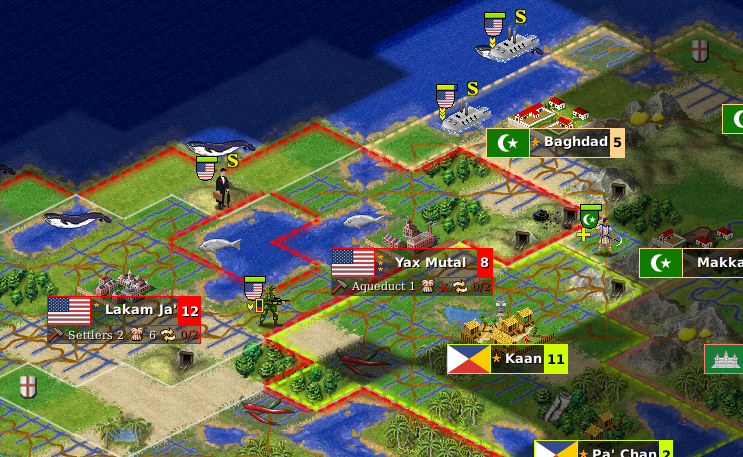
\includegraphics[width=\textwidth]{images/freeciv-example.png}
	\end{columns}

\end{frame}

\begin{frame}
\frametitle{Tipos de terrenos en Freeciv}

\begin{itemize}
	\item Hay \textcolor{UDCpink}{12 tipos de terreno}, con posibles bonificaciones.
\end{itemize}

\vspace{0.5em}

\centering
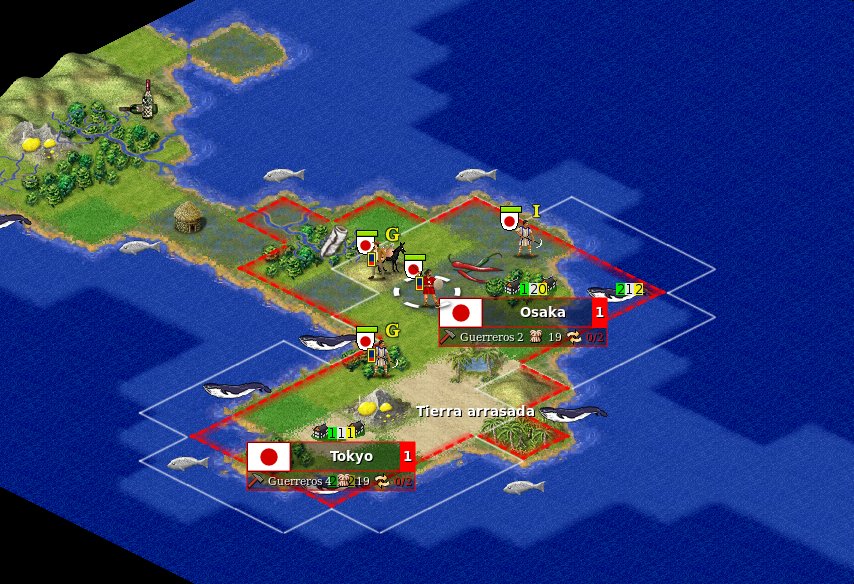
\includegraphics[width=0.8\textwidth]{images/ejemplo-partida.png}
\end{frame}


\begin{frame}
\frametitle{Objetivos del proyecto}

Para este proyecto:

\vspace{1em}

\begin{itemize}
	\item<1-> Se definirá un \textcolor{UDCpink}{modelo declarativo} del escenario para Freeciv usando \textcolor{UDCpink}{\itshape Answer Set Programming}.
	
	\vspace{1em}
	
	\item<2-> Se construirá una pequeña \textcolor{UDCpink}{herramienta gráfica} con la que manipular el escenario.
	
	\vspace{1em}
	
	\item<3-> Eficiencia: reducir o podar el número de combinaciones posibles.
\end{itemize}

\end{frame}

	
	\begin{frame}
	\frametitle{Índice}
		\tableofcontents
	\end{frame}
	
	\AtBeginSection[]
	{
	\begin{frame}
	\frametitle{Índice}
	\tableofcontents[currentsection]
	\end{frame}
	}
	
	\section{Answer Set Programming}
	\begin{frame}
	\frametitle{Answer Set Programming}

	\begin{itemize}
		\item<1-> Paradigma enfocado a la \textcolor{UDCpink}{resolución declarativa} de problemas con complejidad \textcolor{UDCpink}{\textit{NP-hard}}.
		
		\vspace{0.5em}
		
		\item<2-> Combina un \textcolor{UDCpink}{lenguaje simple} (predicados y reglas) con el que modelar problemas lógicos y \textcolor{UDCpink}{herramientas de alto rendimiento}.
	\end{itemize}

	\vspace{0.5em}
	
	\pause[3]
	
	\centering
	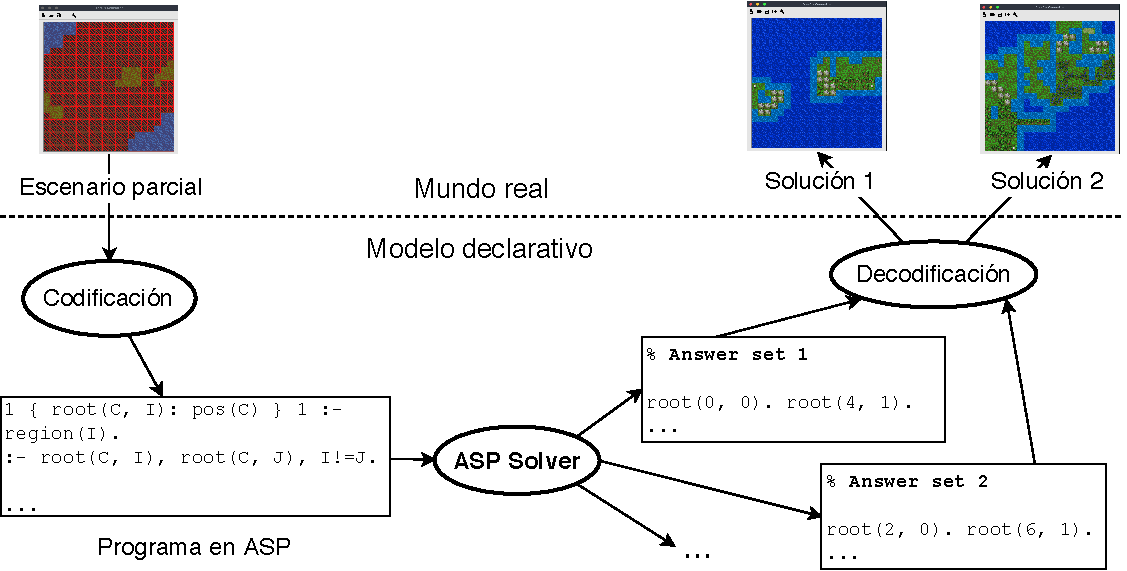
\includegraphics[width=0.9\textwidth]{images/funcionamiento-asp.pdf}
	
\end{frame}

\begin{frame}
\frametitle{Generación del escenario}

\begin{columns}
	\column{0.6\textwidth}
	\begin{itemize}
		\item<1-> Generar todo el terreno a la vez es \textcolor{UDCpink}{inviable}.
		
		\vspace{0.5em}
		
		\item<2-> Se divide el mapa en \textcolor{UDCpink}{cuadrantes} y \textcolor{UDCpink}{regiones}.
		
		\vspace{0.5em}
		
		\begin{itemize}
			\item<2-> Un cuadrante es un grupo de celdas
		\end{itemize}
		
		\begin{enumerate}
			\item<3-> Se genera regiones, que son grupos de cuadrantes conectados entre sí.
			
			\vspace{0.5em}
			
			\item<4-> Se detalla el terreno de cada región, formando islas.
		\end{enumerate}
		
		\vspace{0.5em}
		\item<5-> Los módulos son \textcolor{UDCpink}{independientes}. No necesitan toda la información del problema.
	\end{itemize}
	
	\column{0.4\textwidth}
	\centering
	\begin{overprint}
		\onslide<3>\centering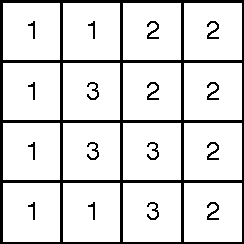
\includegraphics[width=0.9\textwidth]{images/regiones.pdf}
		\onslide<4-|handout:0>\centering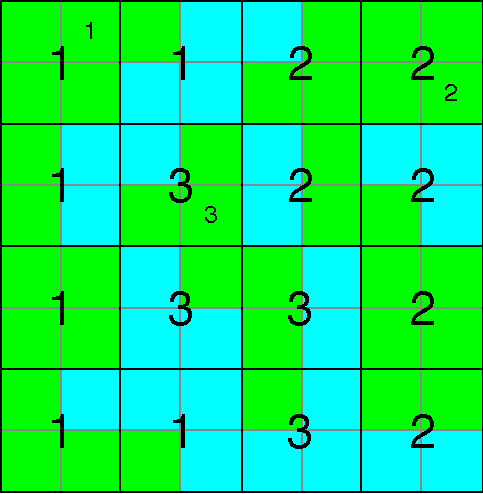
\includegraphics[width=0.9\textwidth]{images/celdas.pdf}
	\end{overprint}
\end{columns}
\end{frame}

\begin{frame}
\frametitle{Ejemplo de algunos predicados usados}

\begin{table}
	\def\arraystretch{1.5}
	\centering
	\begin{tabular}{l p{0.6\textwidth}}
		\hline
		\texttt{root(C, I)} & Cuadrante inicial \texttt{C} de la región \texttt{I}. \\
		\hline
		\texttt{pos(C)} & Posición \texttt{C} de un cuadrante. \\
		\hline
		\texttt{reached(C, I)} & Cuadrante \texttt{C} que ha sido alcanzado. \\
		\hline
		\texttt{adj(C, D)} & Posiciones adyacentes \texttt{C} y \texttt{D} en la cuadrícula. \\
		\hline
		\texttt{land(C)} & Celda \texttt{C} definida como tierra. \\
		\hline
		\texttt{mountain(C)} & Celda \texttt{C} definida como montaña. \\
		\hline
	\end{tabular}
\end{table}

\end{frame}

\begin{frame}
	\frametitle{Ejemplo de algunas reglas lógicas}
	
	\begin{block}{Generación del cuadrantes}		
	\vspace{1em}
	\hspace{2em}\texttt{reached(C, I) :- root(C, I).}
	
	\vspace{1em}
	
	\pause
	
	\hspace{2em}\texttt{0 \{ reached(C, I) \} 1 :- region(I), reached(D, I),}
	
	\hspace{4em}\texttt{adj(D, C), not existsanother(C, I).}
	
	\vspace{1em}
	
	\pause
	
	\hspace{2em}\texttt{1 \{ root(C, I): pos(C) \} 1 :- region(I).}
	
	\vspace{1em}
	
	\pause
	
	\hspace{2em}\texttt{:- root(C, I), root(C, J), region(I), region(J), I!=J.}
	\vspace{1em}
	\end{block}
	
\end{frame}

\begin{frame}
	\frametitle{Ejemplo de algunas reglas lógicas}

	\begin{columns}
	
	\column{0.6\textwidth}
	\begin{block}{\small Generación del cuadrantes}
		\small
		
		\vspace{1em}
		\hspace{1em}\texttt{reached(C, I) :- root(C, I).}
		
		\vspace{1em}
		
		\hspace{1em}\texttt{0 \{ reached(C, I) \} 1 :- }
		
		\hspace{3em}\texttt{region(I), reached(D, I),}
		
		\hspace{3em}\texttt{adj(D, C),}
		
		\hspace{3em}\texttt{not existsanother(C, I).}
		
		\vspace{1em}
		
		\hspace{1em}\texttt{1 \{ root(C, I): pos(C) \} 1 :-}
		
		\hspace{3em}\texttt{region(I).}
		
		\vspace{1em}
		
		\hspace{1em}\texttt{:- root(C, I), root(C, J),}
		
		\hspace{3em}\texttt{region(I), region(J), I!=J.}
		\vspace{1em}
	\end{block}
	
	\column{0.4\textwidth}
	\begin{overprint}
		\onslide<1>\centering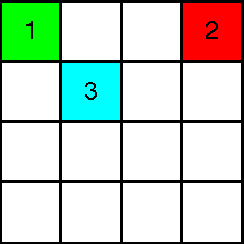
\includegraphics[width=0.9\textwidth]{images/expansion-1.pdf}
		\onslide<2|handout:0>\centering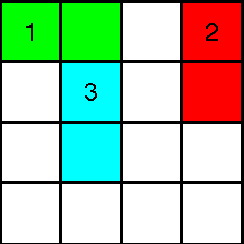
\includegraphics[width=0.9\textwidth]{images/expansion-2.pdf}
		\onslide<3|handout:0>\centering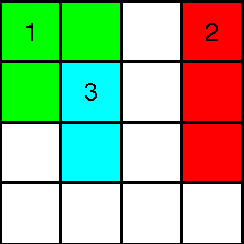
\includegraphics[width=0.9\textwidth]{images/expansion-3.pdf}
		\onslide<4|handout:0>\centering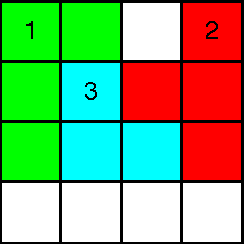
\includegraphics[width=0.9\textwidth]{images/expansion-4.pdf}
		\onslide<5|handout:0>\centering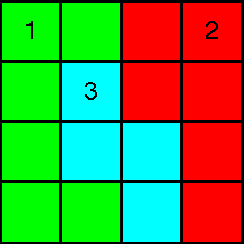
\includegraphics[width=0.9\textwidth]{images/expansion-5.pdf}
	\end{overprint}
	
	\end{columns}

\end{frame}

\begin{frame}
\frametitle{Generación de biomas y de puntos de inicio}

\begin{columns}
	\column{0.6\textwidth}
	
	\begin{itemize}
		\item<1-> \textcolor{UDCpink}{Generación de biomas}:
		
		\vspace{0.5em}
		
		\begin{itemize}
			\item<1-> Un bioma es una zona con el \textcolor{UDCpink}{mismo tipo de terreno}.
			
			\vspace{0.5em}
			
			\item<2-> Misma forma que la generación de islas, salvo que se pueden \textcolor{UDCpink}{pegar}.
		\end{itemize}
	\end{itemize}
	
	\column{0.4\textwidth}
	\centering
	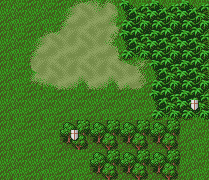
\includegraphics[width=0.6\textwidth]{images/biomas.png}
	
\end{columns}

\vspace{1em}

\begin{itemize}
	\item<3-> \textcolor{UDCpink}{Generación de puntos de inicio}:
	
	\vspace{0.5em}
	
	\begin{itemize}
		\item<3-> Se escoge N celdas de tierra para los jugadores.
		
		\vspace{0.5em}
		
		\item<4-> Para estos puntos se añaden preferencias:
		
		\vspace{0.5em}
		\begin{itemize}
			\item<4-> \textcolor{UDCpink}{Minimizar la distancia al agua}.
			
			\vspace{0.5em}
			
			\item<5-> \textcolor{UDCpink}{Maximizar la distancia a las montañas}.
		\end{itemize}
	\end{itemize}
\end{itemize}

\end{frame}
	
	\section{Demostración}
	
	\section{Trabajo desarrollado}
	\begin{frame}
\frametitle{Arquitectura del sistema}

\begin{itemize}
	\item<1-> \textcolor{UDCpink}{\itshape Front-end}: Creado en \textcolor{UDCpink}{LÖVE}, usa un modelo MVC que usa una interfaz gráfica en modo inmediato.
	
	\vspace{0.5em}
	
	\item<2-> \textcolor{UDCpink}{\itshape Back-end}: Creado en \textcolor{UDCpink}{Lua} (con API de clingo) y \textcolor{UDCpink}{ASP}, usa un modelo en \textit{pipeline}.
\end{itemize}

\pause[3]

\begin{center}
	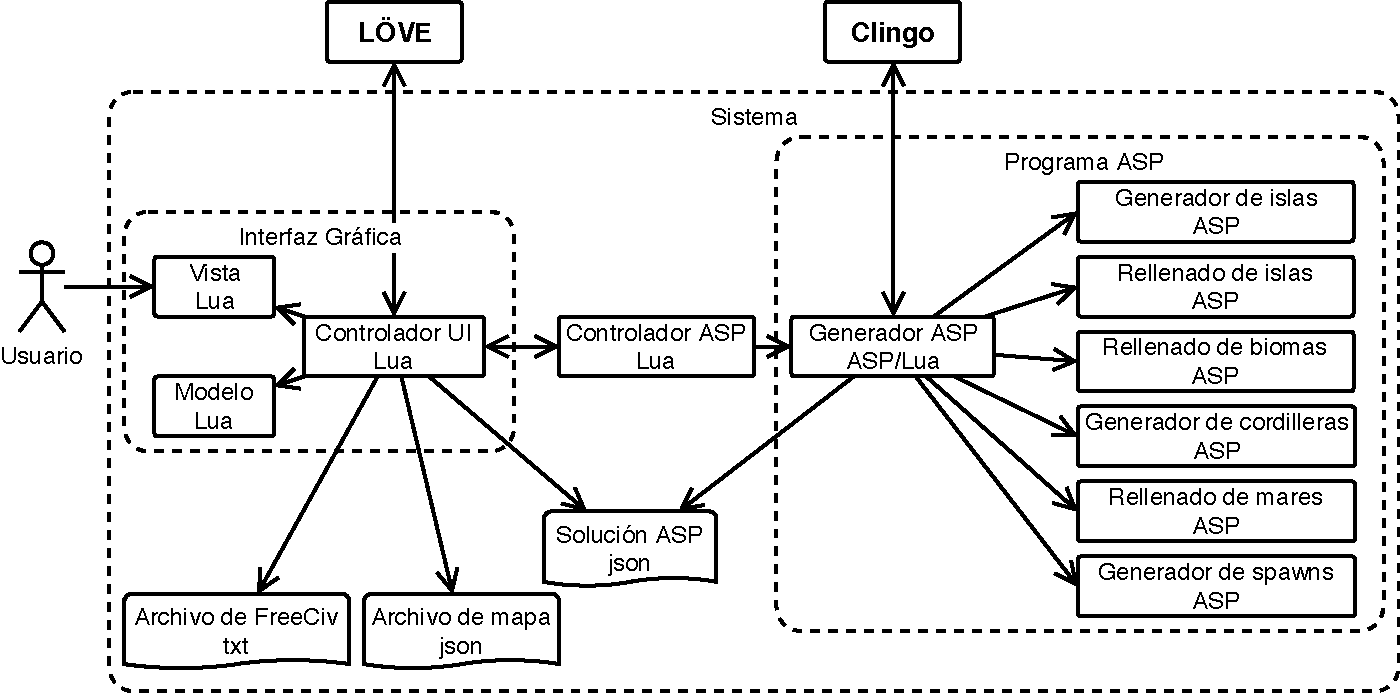
\includegraphics[width=.95\textwidth]{images/arquitectura-completa.pdf}
\end{center}

\end{frame}

\begin{frame}
\frametitle{Proceso de ingeniería}

\begin{itemize}
	\item<1-> Metodología: \textcolor{UDCpink}{desarrollo iterativo incremental y evolutivo}.
	
	\vspace{0.5em}
	
	\item<2-> Se ha usado herramientas de \textcolor{UDCpink}{uso libre y gratuitas} para el desarrollo del proyecto.
	
	\vspace{0.5em}
	
	\item<3-> El coste total del proyecto asciende a \textcolor{UDCpink}{\EUR{3720.00}}.
	
	\vspace{0.5em}	
\end{itemize}

\pause[4]

\centering
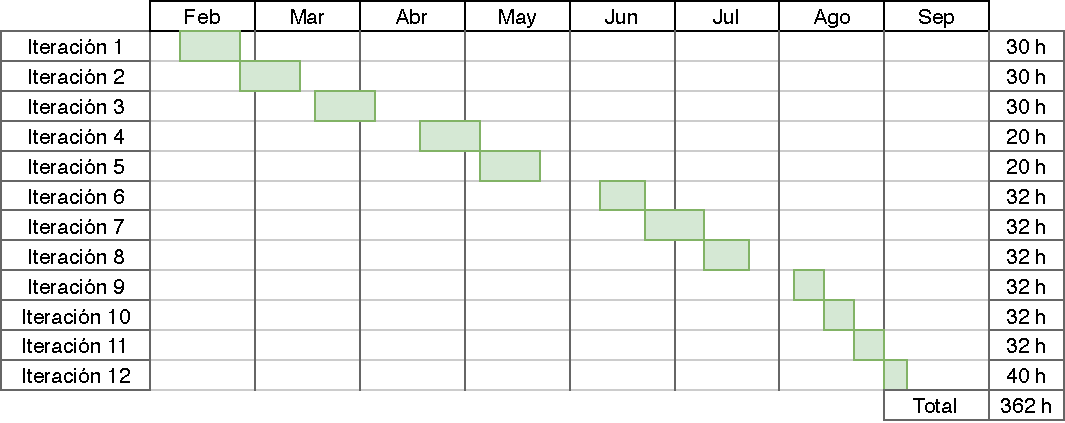
\includegraphics[width=\textwidth]{images/gantt.pdf}

\end{frame}

	\section{Evaluación}
	En este capítulo se analizará los resultados obtenidos en el proceso de evaluación del sistema. Para la planificación de las pruebas se ha optado por el uso de una herramienta de integración continua en donde se corren tanto pruebas de unidad a las partes del modelo de la interfaz gráfica, así como a los distintos módulos de los programas lógicos. \\

Además se ha usado un programa escrito en C\# para la ejecución de pruebas de rendimiento o \textit{benchmarks} el cual solo usa el módulo clingo para evitar el uso de la interfaz gráfica. En todas estas pruebas se ha añadido a las pruebas la restricción de que el cómputo del mapa solo puede durar como máximo cinco minutos, matando el proceso en caso de superar este tiempo y pasando a la siguiente prueba. Con esto podemos indicar cuales son las configuraciones que dan una experiencia pobre al usuario. \\

A continuación se describen los resultados obtenidos de estas pruebas de rendimiento con distintos parámetros. \\

\section{Tamaño de los mapas}

TODO

	\section{Conclusiones}
	En este proyecto se ha enmarcado en el área de la representación del conocimiento. En especial, hemos construido una herramienta declarativa con la que elaborar, mediante programación lógica, polígonos industriales. Esto nos ha permitido crear una herramienta que, en manos de un experto, puede automatizar procesos de construcción de nuevos entornos industriales. Además, al apoyarnos en una herramienta de simulación como es \cities, podemos simular distintas carga de tráfico, una vez generado el polígono. \\

Como ya hemos comentado, gracias al uso de una herramienta declarativa, y de que la parte de definición del programa lógico es externo al algoritmo de búsqueda de modelos estables; un experto en construcción urbanística o de diseño de plantas industriales podría modificar o añadir reglas a su antojo para que la herramienta se adaptara lo máximo posible a su forma de trabajar. Además puede servir como base de datos en un futuro para guardar el tipo de estilo de expertos. \\

Otra parte importante de este trabajo es la construcción del binding de Clingo para el lenguaje de programación C\#. Aún no siendo el objetivo de este proyecto, al ser una biblioteca creada de forma desacoplada del proyecto principal, permite que más personas puedan usar las herramientas de Clingo, en este caso en proyectos creados para .NET. Esto permite una difusión mayor de la programación lógica, y en concreto de Answer Set Programming, para sistemas en los que posiblemente no se hubiera planteado hasta ahora como solución. \\

Para finalizar, este trabajo nos ha permitido ver como funciona un motor de videojuegos tan importante como lo es Unity, y en concreto como incorporar nuevas funcionalidades para un software que su fabricante no tenía pensado hasta ahora. Esto puede servir de gran ayuda para personas que quieran expandir su forma de jugar con un videojuego, además de servir de ejemplo y documentación para gente que esté pensando en entrar en el mundo del desarrollo de videojuegos.

\section{Trabajo futuro}

Con la finalización de este trabajo, se pueden sugerir diferentes líneas de trabajo futuro:

\begin{itemize}
	\item Permitir la generación de edificios de DLCs de \cities como \textit{Industries} o \textit{Sunset Harbor}, añadiendo las mecánicas de procesado de recursos. Además se podría incluir la generación de zonas de aparcamiento, parques y zonas verdes.
	\item Añadir más funcionalidades que nos permite clingo, como reglas de minimización y/o maximización, que permitan crear problemas de optimización a la hora de generar polígonos industriales. Además se podría añadir pesos a las reglas para permitir una generación más personalizada en función de lo que nos comente un experto sobre la construcción de polígonos industriales.
	\item Añadir reglas que permitan también la generación de las topologías de carreteras, pudiendo definir de forma declarativa las distribuciones e incluso unificando el proceso de generación.
	\item Mejorar la usabilidad de la herramienta, permitiendo marcar zonas a mano alzada o con distintas zonas y que tengan en cuenta el terreno. Además se podría incluir nuevas opciones para indicar, por ejemplo, la temática de los edificios a construir o prohibir la generación de un tipo concreto de edificio.
	\item Añadir información externa a la zona a construir, pudiendo unir de forma automática a autopistas o favoreciendo la conexión con zonas ya construidas.
\end{itemize}

	\begin{frame}
		\vbox{}
		\vspace{0.25em}
		\begin{centering}
			{\usebeamercolor[fg]{titlegraphic}\inserttitlegraphic\par}
			\vspace{0.5em}
			\begin{beamercolorbox}[sep=8pt,center,rounded=true]{title}
				\usebeamerfont{title}\inserttitle\par%
				\ifx\insertsubtitle\@empty%
				\else%
				\vspace{0.25em}
				{\usebeamerfont{subtitle}\usebeamercolor[fg]{subtitle}\insertsubtitle\par}%
				\fi%     
			\end{beamercolorbox}%
			\vfill
			\begin{beamercolorbox}[sep=8pt,center]{author}
				\usebeamerfont{author}\insertauthor
			\end{beamercolorbox}
			\vspace{0.5em}
			{\Large\textcolor{UDCpink}{¡Gracias por su atención!}\par}
			\vspace{0.5em}
			\begin{beamercolorbox}[sep=8pt,center]{institute}
				\usebeamerfont{institute}\insertinstitute
			\end{beamercolorbox}
			\begin{beamercolorbox}[sep=8pt,right]{date}
				\itshape\usebeamerfont{date}\insertdate
			\end{beamercolorbox}
		\end{centering}
		\vspace{0.25em}
	\end{frame}

	\begin{frame}
	\frametitle{Ejemplo de la biblioteca de Clingo}
	
	\begin{block}{Añadir restricciones al programa}
		\ttfamily \footnotesize
		
		\#script(lua)
		
		\textbf{function} main(prog)
		
		\hspace{2em} \textit{\textendash\textendash Genero las regiones}
		
		\hspace{2em} \textbf{for} i = 0, c\_regions-1 \textbf{do}
		
		\hspace{4em} \textit{\textendash\textendash Hace grounding del programa lógico}
		
		\hspace{4em} prog:ground(\{\{''base'', \{\}\}, \{''generate'', \{i\}\}\})
		
		\hspace{4em} \textit{\textendash\textendash Obtengo un manejador de la solución}
		
		\hspace{4em} handle = prog:solve({yield=true})
		
		\vspace{1em}
		
		\hspace{4em} \textbf{local} restrictions = '' ''
		
		\hspace{4em} \textit{\textendash\textendash Recorre los modelos de la solución}
		
		\hspace{4em} \textbf{for} model \textbf{in} handle:iter() \textbf{do}
		
		\hspace{6em} \textit{\textendash\textendash Añado las restricciones}
		
		\hspace{6em} \textbf{if} \#restrictions \textasciitilde{}= 0 \textbf{then}
		
		\hspace{8em} prog1:load(''resources/restrictions.lp'')
		
		\hspace{6em} \textbf{end}
		
		\hspace{6em} ...
		
	\end{block}
	\end{frame}
	
	\begin{frame}
	\frametitle{Ejemplo de la biblioteca de Clingo}
	
	\begin{block}{Añadir restricciones al programa}
	\ttfamily \footnotesize
	
	\hspace{6em} \textbf{for} m \textbf{in} handle:iter() \textbf{do}
	
	\hspace{8em} \textbf{for} row\_str, col\_str, contain \textbf{in} string.gmatch(tostring(model), 	''cell\%(p\%((\%d+),(\%d+)\%),(\%l+)\%)'') \textbf{do}
	
	\hspace{10em} \textbf{if} contain == "l"  \textbf{then}
	
	\hspace{12em} lands = lands .. '' land(p(''..row\_str..'',''..col\_str..'')).''
	
	\hspace{12em} restrictions = restrictions .. check\_restrictions(row, col, i)
	
	\hspace{10em} \textbf{end}
	
	\hspace{8em} \textbf{end}
	
	\vspace{1em}
	
	\hspace{8em} df = io.open(''resources/restrictions.lp'', ''w+'')
	
	\hspace{8em} df:write(restrictions)
	
	\hspace{8em} df:flush()
	
	\hspace{8em} df:close()
	
	\hspace{6em} \textbf{end}
	
	\hspace{4em} \textbf{end}
	
	\hspace{2em} \textbf{end}
	
	\textbf{end}
	
	\#end.
	\end{block}
	\end{frame}

	\begin{frame}
	\frametitle{Ejecución del módulo Clingo}
	
	\centering
	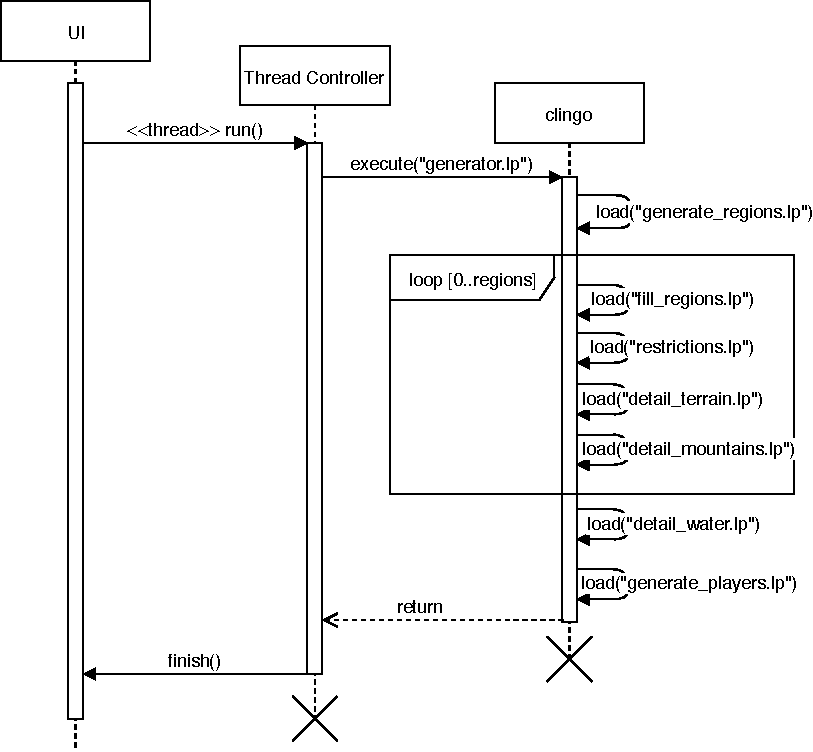
\includegraphics[width=0.6\textwidth]{images/diagrama-secuencia.pdf}
	
	\end{frame}

	\begin{frame}
	\frametitle{Ejemplo de generación 20x20}
	
	\centering
	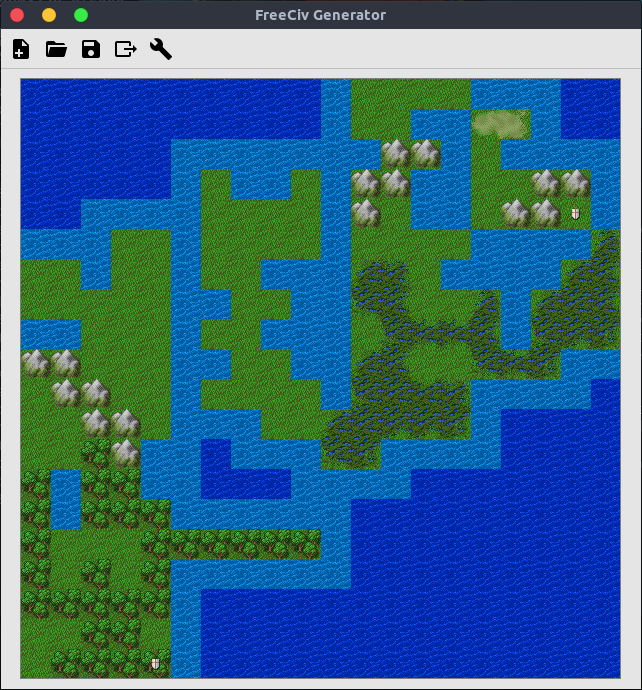
\includegraphics[width=0.6\textwidth]{images/ejemplo-20-20.png}
	
	\end{frame}

	\begin{frame}
	\frametitle{Ejemplo de generación 30x30}
	
	\centering
	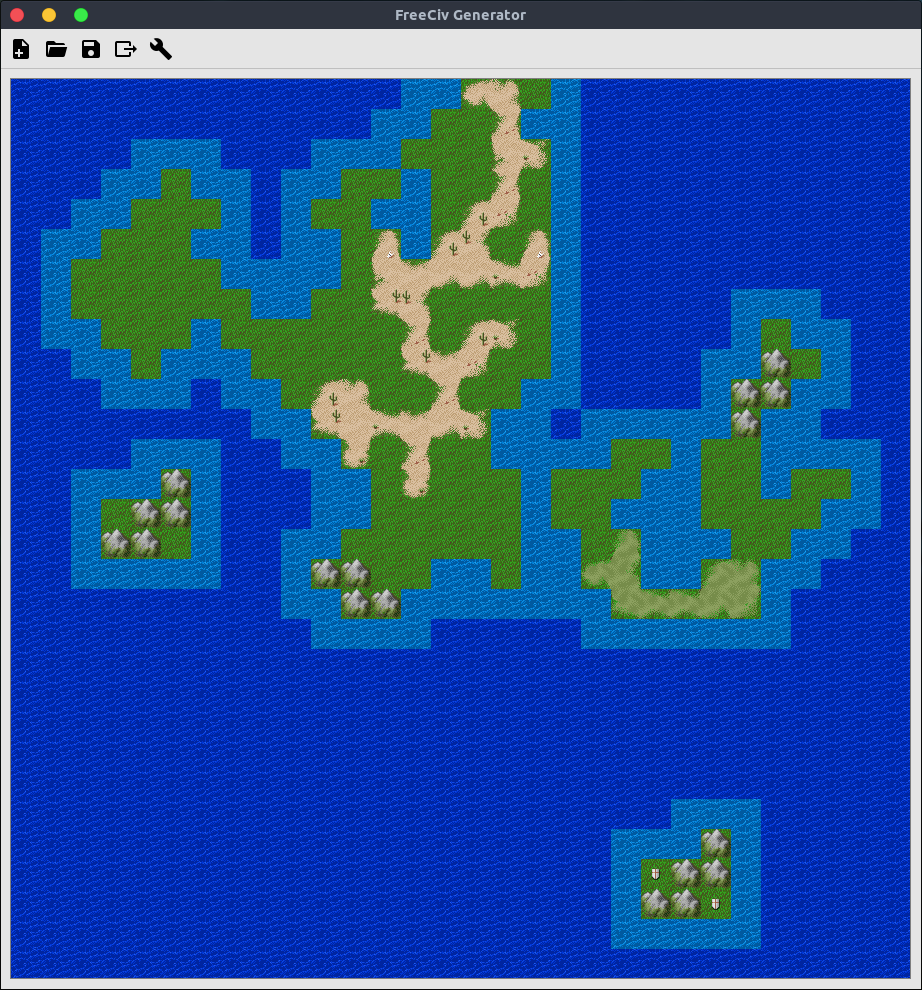
\includegraphics[width=0.6\textwidth]{images/ejemplo-30-30.png}
	
	\end{frame}

\end{document}